\begin{exercise}\label{ex:020301}
    Construct a syntax directed translation scheme that translates arithmetic 
    expressions from infix notation into prefix notation in which an operator 
    appears before its operands; e.g., $-xy$ is the prefix notation for $x - y$.
    Give annotated parse trees for the inputs \texttt{9-5+2} and \texttt{9-5*2}.
\end{exercise}
\begin{solution}\label{sol:020301}
    The translation scheme is given below.
    \begin{align*}
            E &\yld \cbrak{\text{print(`\texttt{+}')}}\ E\ \texttt{+}\ T\ |\ \cbrak{\text{print(`\texttt{-}')}}\ E\ \texttt{-}\ T\ |\ T \\
            T &\yld \cbrak{\text{print(`\texttt{*}')}}\ T\ \texttt{*}\ F\ |\ \cbrak{\text{print(`\texttt{/}')}}\ T\ \texttt{/}\ F\ |\ F \\
            F &\yld \cbrak{\text{print(id)}}\ id\ |\ \cbrak{\text{print(num)}}\ num\ |\ (E)
    \end{align*}
    The parse trees for the inputs \texttt{9-5+2} and \texttt{9-5*2} are shown 
    in \autoref{fig:020301a} and \autoref{fig:020301b} respectively.
    \begin{figure}[!ht]
    \centering
    \begin{tikzpicture}
        [
            level distance = 3em, 
            level 1/.style={sibling distance=8em},
            level 2/.style={sibling distance=4em},
        ]
        \node {$E$}
        child {
            node {print(`\texttt{+}')} edge from parent[dashed]
        }
        child {
            node {$E$}
            child {
                node {print(`\texttt{-}')} edge from parent[dashed]
            }
            child {
                node {$E$}
                child {
                    node {$T$}
                        child {
                        node {$F$}
                        child {
                            node {print(`\texttt{9}')} edge from parent[dashed]
                        }
                        child {node{\texttt{9}}}
                    }
                }
            }
            child {node {\texttt{-}}}
            child {
                node {$T$}
                child {
                    node {$F$}
                    child {
                        node {print(`\texttt{5}')} edge from parent[dashed]
                    }
                    child {node {\texttt{5}}}
                }
            }
        }
        child {node {\texttt{+}}}
        child {
            node {$T$}
            child {
                node {$F$}
                child {
                    node {print(`\texttt{2}')} edge from parent[dashed]
                }
                child {node {\texttt{2}}}
            }
        }
        ;
    \end{tikzpicture}
    \caption{Parse tree for the input \texttt{9-5+2} for \cref{ex:020301}.}
    \label{fig:020301a}
\end{figure}

    \begin{figure}[!ht]
    \centering
    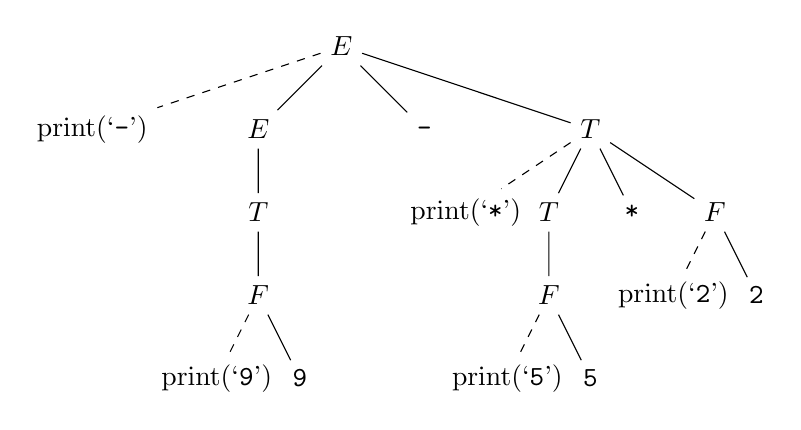
\begin{tikzpicture}
        [
            level distance = 3em, 
            level 1/.style={sibling distance=6em},
            level 2/.style={sibling distance=3em},
        ]
        \node {$E$}
        child {
            node {print(`\texttt{-}')} edge from parent[dashed]
        }
        child {
            node {$E$}
            child {
                node {$T$}
                    child {
                    node {$F$}
                    child {
                        node {print(`\texttt{9}')} edge from parent[dashed]
                    }
                    child {node{\texttt{9}}}
                }
            }
        }
        child {node {\texttt{-}}}
        child {
            node {$T$}
            child {
                node {print(`\texttt{*}')} edge from parent[dashed]
            }
            child {
                node {$T$}
                child {
                    node {$F$}
                    child {node {print(`\texttt{5}')} edge from parent[dashed]}
                    child {node {\texttt{5}}}
                }
            }
            child {node {\texttt{*}}}
            child {
                node {$F$}
                child {node {print(`\texttt{2}')} edge from parent[dashed]}
                child {node {\texttt{2}}}
            }
        }
        ;
    \end{tikzpicture}
    \caption{Parse tree for the input \texttt{9-5*2} for \cref{ex:020301}.}
    \label{fig:020301b}
\end{figure}
\end{solution}